\chapter{The Issue Unit}\label{chapter:issue}

The issue window holds dispatched micro-ops that have not yet executed.  When all of the operands for the micro-op are ready, the issue slot sets its ``request" bit high.  The issue select logic then chooses to issue a slot which is asserting its ``request" signal.  Once a micro-op is issued, it is removed from the issue window to make room for more dispatched instructions. 

BOOM uses a ``unified" issue window - all instructions of all types (integer, floating point, memory) are placed into a single issue window. 

\section{Speculative Issue}

Although not yet supported, future designs may choose to speculatively issue micro-ops for improved performance (e.g., speculating that a load instruction will hit in the cache and thus issuing dependent micro-ops assuming the load data will be available in the bypass network). In such a scenario, the issue window cannot remove speculatively issued micro-ops until the speculation has been resolved. If a speculatively-issued micro-op failure occurs, then all issued micro-ops that fall within the speculated window must be killed and retried from the issue window. More advanced techniques are also available.

\section{Issue Slot}

Figure \ref{fig:riscv-boom_issue_slot} shows a single issue slot from the {\em Issue Window}.\footnote{Conceptually, a bus is shown for implementing the driving of the signals sent to the {\em Register Read} Stage.  In reality BOOM actually uses muxes.}

Instructions are {\em dispatched} into the {\em Issue Window}.  From here, they wait for all of their operands to be ready (``p" stands for {\em presence} bit, which marks when an operand is {\em present} in the register file).  

Once ready, the {\em issue slot} will assert its ``request" signal, and wait to be {\em issued}.  

\begin{figure}[ht]
	\centering
	\centerline{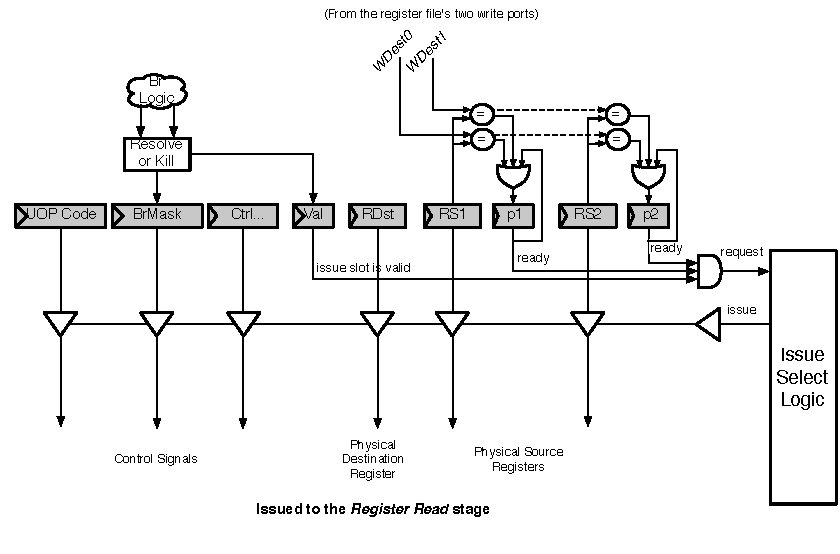
\includegraphics[scale =1.0] {figures/issue_slot}}
	\caption{ \small A single issue slot from the Issue Window.}
	\label{fig:riscv-boom_issue_slot}
\end{figure}

\section{Issue Select Logic}

Each issue select logic port is a static-priority encoder that picks that first available micro-op in the issue window.  Each port will only schedule a micro-op that its port can handle (e.g., floating point micro-ops will only be scheduled onto the port governing the Floating Point Unit). This creates a cascading priority encoder for ports that can schedule the same micro-ops as each other. 

If a functional unit is unavailable, it de-asserts its available signal and instructions will not be issued to it (e.g., an un-pipelined divider). 

\section{Un-ordered Issue Window}

There are two scheduling policies available in BOOM.

The first is a R10K-style un-ordered issue window.\cite{mipsr10k}  Dispatching instructions are placed into the first available issue window slot and remain there until they are {\em issued}.  This can lead to pathologically poor performance, particularly in scenarios where unpredictable branches are placed into the lower priority slots and are unable to be issued until the ROB fills up and the issue window starts to drain.  Because instructions following branches are only {\em implicitly} dependent on the branch, there is no other forcing function that enables the branches to issue earlier, except the filling of the ROB. 

\section{Age-ordered Issue Window}

The second available policy is an age-ordered issue window.  Dispatched instructions are placed into the bottom of the issue window (at lowest priority). Every cycle, every instruction is shifted upwards (the issue window is a ``collapsing queue").  Thus, the oldest instructions will have the highest issue priority.  While this increases performance by scheduling older branches and older loads as soon as possible, it comes with a potential energy penalty as potentially every issue window slot is being read and written to on every cycle. 

